% !Mode:: "TeX:UTF-8"
% !TEX program  = xelatex


% \documentclass{cumcmthesis}
\documentclass[withoutpreface,bwprint]{cumcmthesis} %去掉封面与编号页，电子版提交的时候使用。


\usepackage[framemethod=TikZ]{mdframed}
\usepackage{url}   % 网页链接
\usepackage{subcaption} % 子标题

\makeatletter
\pdfstringdefDisableCommands{%
  \let\leavevmode@ifvmode\relax
  \def\kern#1{}%
}
\makeatother

\title{柱面反射艺术的数学建模与优化设计}
\tihao{A}
\baominghao{4321}
\schoolname{XX大学}
\membera{ }
\memberb{ }
\memberc{ }
\supervisor{ }
\yearinput{2020}
\monthinput{08}
\dayinput{22}

\begin{document}
 
 \maketitle
 \begin{abstract}

     \par
     柱面反射艺术（Catoptric Anamorphosis）利用光学反射原理，将纸面上的不规则畸变图像在圆柱形镜面中还原为具有实际意义的视觉图案 。本文旨在探究该错觉艺术背后的深层数学与光学原理，并建立一套从空间几何映射到多模态视觉优化的完整数学建模方案，以实现自动化、高精度的反射艺术设计。
     \par
     \textbf{针对问题一：}
     本文构建了基于三维空间解析几何的逆向光线追踪模型。首先建立空间直角坐标系，通过设定观察者视点、圆柱镜面方程及虚拟投影平面，联立求解视线射线与圆柱面的二次交点方程 。随后，利用交点处的法向量与光学反射定律，推导出反射光线并计算其与水平纸面的映射坐标 。为克服传统正向映射中非线性拉伸导致的“像素空洞”缺陷，本文采用基于散点网格的双线性插值算法，成功设计并生成了高精度的蒙娜丽莎与卡通猫预畸变图案，并给出了严格适配 A4 幅面的物理参数配置。
     \par
     \textbf{针对问题二 ：}
        在构建的几何模型基础上，本文设计了一个多模态联合感知寻优算法。该算法结合了遗传算法与梯度下降法，通过定义适应度函数来评估生成图案的视觉质量与稳定性。针对拓扑视场分割与超定方程冲突问题，本文引入了基于图论的分割策略和正则化项，有效约束了优化过程中的解空间，确保了错觉艺术图案的自动化、高精度生成。
     \par
    \textbf{针对问题三：}
    





\keywords{\quad 曲面\quad  光学\quad   几何\quad   anamorphosis \quad 墨卡托投影 \quad 光线追踪}
\end{abstract}

%目录  2019 明确不要目录，我觉得这个规定太好了
%\tableofcontents

%\newpage

\section{问题重述}
\subsection{问题背景}
“柱面反射艺术”巧妙结合了严密的几何学与人类视觉感知。艺术家在平面上绘制高度扭曲、看似混乱的图案，经过特定圆柱镜面的反射后，却能在特定视角下重组为正常的具象画面。

从数学本质来看，这是一个跨维度的非线性空间连续映射过程。传统手工创作不仅耗时，且在处理图像高频细节时，极易产生“像素空洞”与拉伸失真。

本项目旨在将此复杂的光学过程抽象为精确的计算机数学模型。通过建立从“基于逆向光线追踪的解析几何映射”到“多模态联合感知寻优”的完整方案，不仅解决拓扑视场分割与超定方程冲突问题，实现错觉艺术图案的自动化、高精度生成，更为现代逆向光学设计与视觉加密提供坚实的数学支撑。
\begin{figure}[H]  % [H] = 强制放在当前位置
    \centering     % 图片居中
    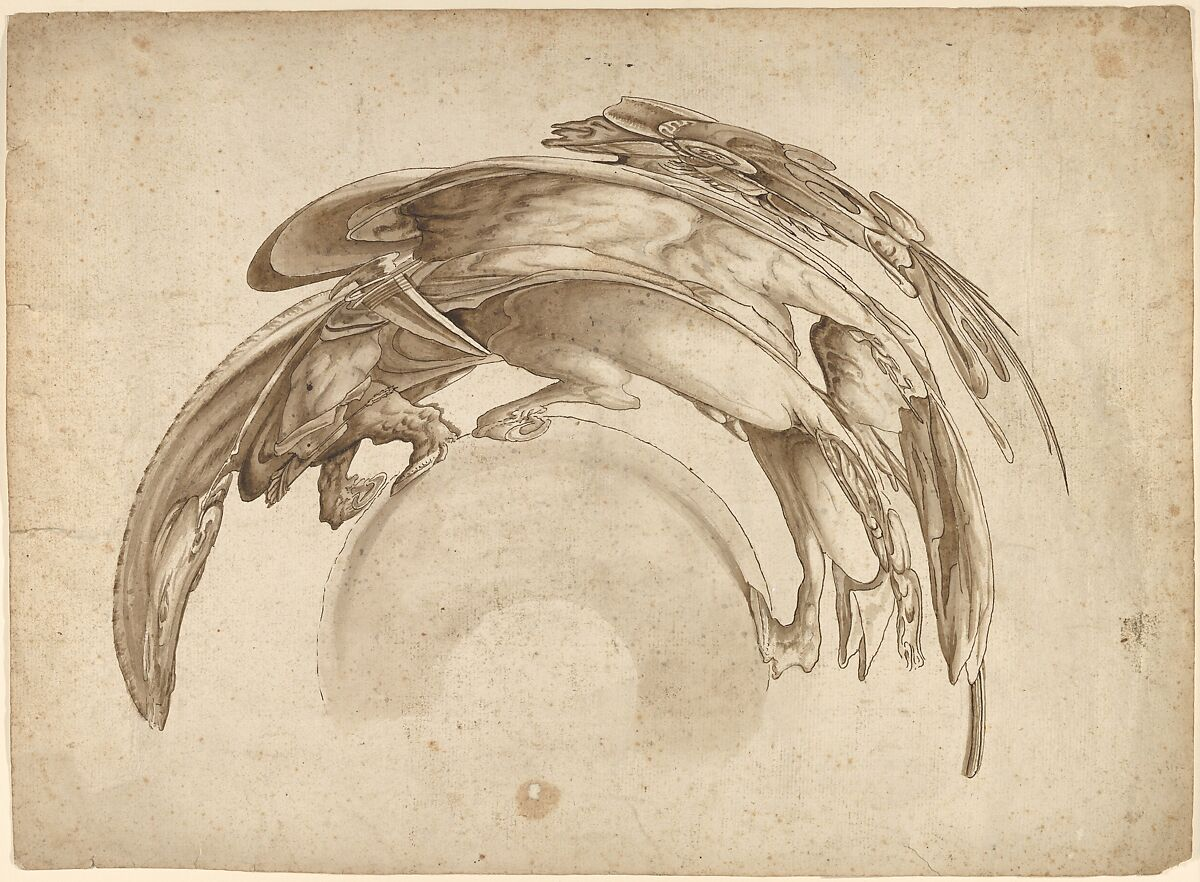
\includegraphics[width=0.8\textwidth]{figures/f1.jpg}
    \caption{Jean François Niceron - Soldier on Horseback in Catoptric Anamorphosis}
    \label{fig:myimage}  % 用于交叉引用
\end{figure}
\subsection{问题提出}
基于上述背景，本文将围绕以下三个核心问题展开研究：
\begin{itemize}
    \item \textbf{问题一：} 如何构建一个基于逆向光线追踪的解析几何模型，实现从空间三维坐标到二维纸面坐标的精确映射，解决传统正向映射中非线性拉伸导致的“像素空洞”问题，并成功生成适配 A4 幅面的高精度预畸变图案？
    \item \textbf{问题二：} 在构建的几何模型基础上，如何设计一个多模态联合感知寻优算法，解决拓扑视场分割与超定方程冲突问题，实现错觉艺术图案的自动化、高精度生成？
    \item \textbf{问题三：} 如何通过数学建模与算法优化，提升生成的柱面反射艺术图案的视觉质量与稳定性，确保在实际应用中能够达到预期的艺术效果？
    

\end{itemize}



\section{问题分析}
\subsection{问题一的分析}
\subsection{问题二的分析}
\subsection{问题三的分析}


\section{模型假设}
\begin{enumerate}
  \item  纸张为平面上的一部分，A4 幅面大小,纸张所在的平面为绝对水平的理想二维平面。

  \item 镜面为理想圆柱体的侧面，圆柱体高
度有限，竖直放置,圆柱形镜面为理想的全反射几何柱面，且忽略镜面材料的物理厚度。
 \item 纸张上的图案称为纸面图案，观察者看到的镜面反射图案称为
镜面图案。
  \item 设计时，纸面图案不需要限定为手绘图案，并且可以对镜面图案或纸面
图案进行艺术加工或简化。
\item 假设观察者的视线为一个理想的几何空间点线，且观察者的视点位置固定不变。
\item 假设环境光照均匀且恒定，不考虑圆柱体在纸面上投射的阴影。
\end{enumerate}

\section{符号说明}

\begin{table}[!htbp]
    \caption{标准三线表格}\label{tab:001} \centering
    \begin{tabular}{ccccc}
        \toprule[1.5pt]
        $D$(in) & $P_u$(lbs) & $u_u$(in) & $\beta$ & $G_f$(psi.in)\\
        \midrule[1pt]
        5 & 269.8 & 0.000674 & 1.79 & 0.04089\\
        10 & 421.0 & 0.001035 & 3.59 & 0.04089\\
        20 & 640.2 & 0.001565 & 7.18 & 0.04089\\
        \bottomrule[1.5pt]
    \end{tabular}
\end{table}



\section{模型建立与求解}
\subsection{问题一}
\subsection{问题二}
\subsection{问题三}


\section{参考文献与引用}

参考文献对于一篇正式的论文来说是必不可少的，在建模中重要的参考文献当然应该列出。\LaTeX{}在这方面的功能也是十分强大的，下面进介绍一个比较简单的参考文献制作方法。有兴趣的可以学习 \verb|bibtex| 或 \verb|biblatex| 的使用。

\LaTeX{}的入门书籍可以看《\LaTeX{}入门》\cite{liuhaiyang2013latex}。这是一个简单的引用，用 \verb|\cite{bibkey}| 来完成。要引用成功，当然要维护好 bibitem 了。下面是个简单的例子。

 

%参考文献
\begin{thebibliography}{9}%宽度9
    \bibitem[1]{liuhaiyang2013latex}
    刘海洋.
    \newblock \LaTeX {}入门\allowbreak[J].
    \newblock 电子工业出版社, 北京, 2013.
    \bibitem[2]{mathematical-modeling}
    全国大学生数学建模竞赛论文格式规范 (2020 年 8 月 25 日修改).
    \bibitem{3} \url{https://www.latexstudio.net}
\end{thebibliography}

\newpage
%附录
\begin{appendices}

\section{模板所用的宏包}
\begin{table}[htbp]
    \centering
    \caption{宏包罗列}
    \begin{tabular}{ccccc}
        \toprule
        \multicolumn{5}{c}{模板中已经加载的宏包} \\
        \midrule
        amsbsy & amsfonts & {amsgen} & {amsmath} & {amsopn} \\
        amssymb & amstext & {appendix} & {array} & {atbegshi} \\
        atveryend & auxhook & {bigdelim} & {bigintcalc} & {bigstrut} \\
        bitset & bm    & {booktabs} & {calc} & {caption} \\
        caption3 & CJKfntef & {cprotect} & {ctex} & {ctexhook} \\
        ctexpatch & enumitem & {etexcmds} & {etoolbox} & {everysel} \\
        expl3 & fix-cm & {fontenc} & {fontspec} & {fontspec-xetex} \\
        geometry & gettitlestring & {graphics} & {graphicx} & {hobsub} \\
        hobsub-generic & hobsub-hyperref & {hopatch} & {hxetex} & {hycolor} \\
        hyperref & ifluatex & {ifpdf} & {ifthen} & {ifvtex} \\
        ifxetex & indentfirst & {infwarerr} & {intcalc} & {keyval} \\
        kvdefinekeys & kvoptions & {kvsetkeys} & {l3keys2e} & {letltxmacro} \\
        listings & longtable & {lstmisc} & {ltcaption} & {ltxcmds} \\
        multirow & nameref & {pdfescape} & {pdftexcmds} & {refcount} \\
        rerunfilecheck & stringenc & {suffix} & {titletoc} & {tocloft} \\
        trig  & ulem  & {uniquecounter} & {url} & {xcolor} \\
        xcolor-patch & xeCJK & {xeCJKfntef} & {xeCJK-listings} & {xparse} \\
        xtemplate & zhnumber &       &       &  \\
        \bottomrule
    \end{tabular}%
    \label{tab:addlabel}%
\end{table}%

以上宏包都已经加载过了，不要重复加载它们。

\section{排队算法--matlab 源程序}

\begin{lstlisting}[language=matlab]
kk=2;[mdd,ndd]=size(dd);
while ~isempty(V)
[tmpd,j]=min(W(i,V));tmpj=V(j);
for k=2:ndd
[tmp1,jj]=min(dd(1,k)+W(dd(2,k),V));
tmp2=V(jj);tt(k-1,:)=[tmp1,tmp2,jj];
end
tmp=[tmpd,tmpj,j;tt];[tmp3,tmp4]=min(tmp(:,1));
if tmp3==tmpd, ss(1:2,kk)=[i;tmp(tmp4,2)];
else,tmp5=find(ss(:,tmp4)~=0);tmp6=length(tmp5);
if dd(2,tmp4)==ss(tmp6,tmp4)
ss(1:tmp6+1,kk)=[ss(tmp5,tmp4);tmp(tmp4,2)];
else, ss(1:3,kk)=[i;dd(2,tmp4);tmp(tmp4,2)];
end;end
dd=[dd,[tmp3;tmp(tmp4,2)]];V(tmp(tmp4,3))=[];
[mdd,ndd]=size(dd);kk=kk+1;
end; S=ss; D=dd(1,:);
 \end{lstlisting}

 \section{规划解决程序--lingo源代码}

\begin{lstlisting}[language=c]
kk=2;
[mdd,ndd]=size(dd);
while ~isempty(V)
    [tmpd,j]=min(W(i,V));tmpj=V(j);
for k=2:ndd
    [tmp1,jj]=min(dd(1,k)+W(dd(2,k),V));
    tmp2=V(jj);tt(k-1,:)=[tmp1,tmp2,jj];
end
    tmp=[tmpd,tmpj,j;tt];[tmp3,tmp4]=min(tmp(:,1));
if tmp3==tmpd, ss(1:2,kk)=[i;tmp(tmp4,2)];
else,tmp5=find(ss(:,tmp4)~=0);tmp6=length(tmp5);
if dd(2,tmp4)==ss(tmp6,tmp4)
    ss(1:tmp6+1,kk)=[ss(tmp5,tmp4);tmp(tmp4,2)];
else, ss(1:3,kk)=[i;dd(2,tmp4);tmp(tmp4,2)];
end;
end
    dd=[dd,[tmp3;tmp(tmp4,2)]];V(tmp(tmp4,3))=[];
    [mdd,ndd]=size(dd);
    kk=kk+1;
end;
S=ss;
D=dd(1,:);
 \end{lstlisting}
\end{appendices}

\end{document} 